\chapter{External Memory}

When handling very large texts and indices, the data might not fit into memory any more. In this case some of it must be swapped to the disk, resulting in much greater access times. To analyze the performance of these indices we introduce the \defi{external memory model}{External Memory Model} shown in Figure~\ref{fig:externalMemoryModel}. Here the CPU can only work with data available in the main memory but all executed operations have zero cost. The only costing operation is to load a block from the disk to the main memory. Each of these loads costs one unit. In the following sections we specify the model by two parameters: $B$ is the number of items stored in each block and $M$ is the number of items that fit into the main memory simultaneously.

\begin{figure}[htb]
  \centering
  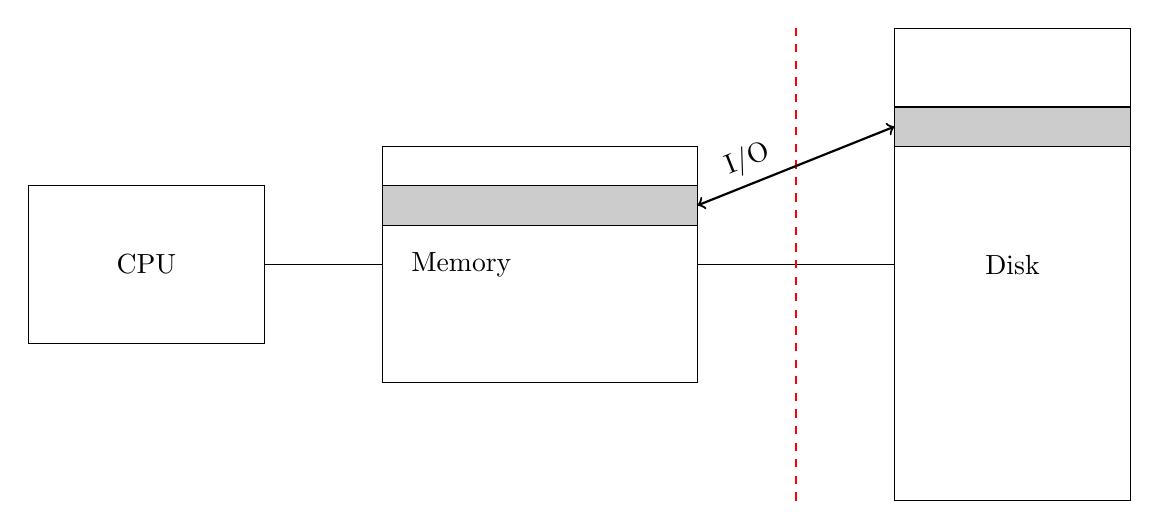
\begin{tikzpicture}
  \draw[fill=black!20!white] (11, 2.5) -- (14, 2.5) -- (14, 3) -- (11, 3) -- cycle;
  \draw[fill=black!20!white] (4.5, 1.5) -- (8.5, 1.5) -- (8.5, 2) -- (4.5, 2) -- cycle;

  \draw (0, 0) -- (3, 0) -- (3, 2) -- (0, 2) -- cycle;
  \draw (4.5, -0.5) -- (8.5, -0.5) -- (8.5, 2.5) -- (4.5, 2.5) -- cycle;
  \draw (11, -2) -- (14, -2) -- (14, 4) -- (11, 4) -- cycle; 

  \draw (3, 1) -- (4.5, 1);
  \draw (8.5, 1) -- (11, 1);
  \draw[red, dashed] (9.75, -2) -- (9.75, 4);
  \draw[thick, <->] (8.5, 1.75) -- (11, 2.75) node[above, sloped, pos=0.3] {I/O}; 

  \node (cpu) at (1.5, 1) {CPU};
  \node (memory) at (5.5, 1) {Memory};
  \node (disk) at (12.5, 1) {Disk};
\end{tikzpicture}

  \caption{Schematic set up of the external memory model.}
  \label{fig:externalMemoryModel}
\end{figure}

\begin{Example}
  Let $T$ be a text of length $n$ and $q$ be a query of size $m$. The I/O complexity for count queries using a suffix array is given by $\mathcal{O}(m\cdot\log\frac{n}{B})$. For this example we used a naive binary search in the suffix array, comparing the query to $\mathcal{O}(\log n)$ suffixes.
\end{Example}

\section{String-B-Tree}

Given is a set $S = \{s_0, \ldots, s_{N - 1}\}$ of $N$ strings of total length $N$. A \emph{prefix count query} asks for the subset of strings starting with a given pattern $P$. We will describe a datastructure to answer prefix count queries efficiently in the external memory model.

\begin{Definition}
  A \defi{String-B-Tree}{String-B-Tree} (\id{SBT}) is a combination of a $B$-tree and a Patricia-trie. The keys of the \id{SBT} are pointers to the text (which is stored in external memory). The keys are stored in the leaves and their order is determined by the lexicographical ordering of the corresponding strings. The inner vertices store the minimal and the maximal keys of their children to allow efficient navigation.
\end{Definition}

Each node $v$ of the \id{SBT} is stored in a disk block and contains an ordered string set $S_v \subset S$. For a $b \in \Theta(B)$ we assume $b \leq \vert S_v \vert \leq 2b$. The leftmost string in $S_v$ is $L(v)$ and the rightmost one is $R(v)$.

To construct the \id{SBT} partition the ordered $S$ into groups of $b$ strings (the last group may have less than $b$ strings). Each group is mapped to a leaf, such that a left-to-right scan of the leaves gives all strings from $S$ in lexicographical order. With each pair $S_j, S_{j+1}$ we associate the longest common prefix $\proc{LCP}(S_j, S_{j+1})$. Each internal node $v$ had $d(v)$ children $u_0, \ldots, u_{d(v) - 1}$ where $\frac{b}{2} \leq d(v) \leq b$ (the root may have from $2$ to $b$ children). Its set $S_v$ is formed by copying the leftmost and rightmost strings of $v$'s children: $S_v = \{L(u_0), R(u_0), \ldots, L(u_{d(v) - 1}), R(u_{d(v) - 1})\}$

\begin{Example}
  Consider the following text where the numbers above each word give the index of its first character. Its \id{STB} is given in Figure~\ref{fig:stringBTree}.
  % Stupid indention is to have the text more or less centered...
  \begin{verbatim}
                           1   1     2     2      3     4
              0 2     8    3   7     3     9      6     2
              i think that the ruddy widow really wants ripe

              4          5   6   6     7    7      8
              7          8   2   6     2    7      4
              watermelon and red roses when winter arrives
  \end{verbatim}

  \begin{figure}[htb]
    \centering
    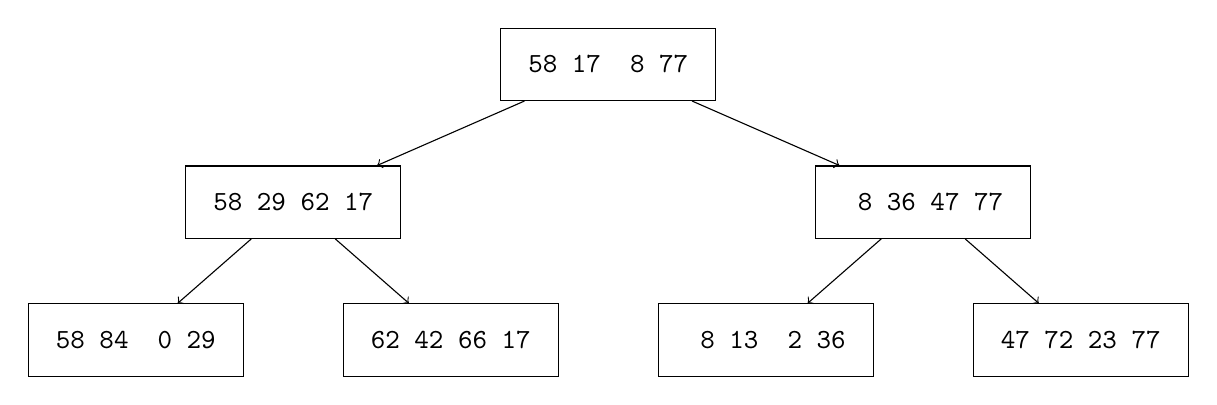
\begin{tikzpicture}
  \node[draw, inner sep=10pt] (root) at (6, 3.5) {\texttt{58~17~~8~77}};
  \node[draw, inner sep=10pt] (l) at (2, 1.75) {\texttt{58~29~62~17}};
  \node[draw, inner sep=10pt] (r) at (10, 1.75) {\texttt{~8~36~47~77}};
  \node[draw, inner sep=10pt] (ll) at (0, 0) {\texttt{58~84~~0~29}};
  \node[draw, inner sep=10pt] (lr) at (4, 0) {\texttt{62~42~66~17}};
  \node[draw, inner sep=10pt] (rl) at (8, 0) {\texttt{~8~13~~2~36}};
  \node[draw, inner sep=10pt] (rr) at (12, 0) {\texttt{47~72~23~77}};

  \draw[->] (root) -- (l);
  \draw[->] (root) -- (r);
  \draw[->] (l) -- (ll);
  \draw[->] (l) -- (lr);
  \draw[->] (r) -- (rl);
  \draw[->] (r) -- (rr);
\end{tikzpicture}

    \caption{The \id{STB} for text $T~=~$\texttt{i think that the ruddy widow really wants ripe and red roses when winter arrives}.}
    \label{fig:stringBTree}
  \end{figure}
\end{Example}

In each node $v$ of the \id{SBT} its string set $S_v$ is stored as a \defi{blind trie}{Blind Trie}. To do this we build a patricia trie over the (binary encoded) strings in $S_v$. We can store the trie in a succinct tree representation, so that it fits into the same memory block and the matching in it does not require further I/Os. For a pattern $P$ we follow the blind search until reaching a leaf. We then check in the text, whether $P$ occurs at the pointer returned by the blind search in the leaf and either stop or proceed with the left or right child.
% TODO (pjungeblut): Add an image showing the blind trie for one of the vertices
%                    Probably do not take the root but one where what happens is
%                    a little bit more interesting.

Assuming that the subtree sizes are stored at each node, count queries for a pattern $P$ then take $\mathcal{O}(\frac{\vert P \vert}{B} + \log_B N)$ time. For locate queries we need to descend to each leaf containing $P$, so the time becomes $\mathcal{O}(\frac{\vert P \vert + Z}{B} + \log_B N)$ where $Z$ is the number of strings in $S$ prefixed by $P$.

The \id{SBT} has $\mathcal{O}(\frac{N}{B})$ leaves and therefore $\mathcal{O}(\frac{N}{B})$ inner nodes. Each node fits into a disk block.

\section{Geometric Burrows-Wheeler-Transformation}

% TODO (pjungeblut): Write section about the geometric Burrows-Wheeler-
%                    Transformation,

